
\section{Requirements}
\label{sec:requirements}


\vitae is a Vaadin Java Web Application, following the Vaadin
architecture 

\subsection{Applications UIs}
\label{sec:applications-uis}

\vitae offers differentiated services to users, dependending on the
role they play inside the application: \textbf{Guest, User, Manager,
  Admin}. The entry point of \vitae is the \textbf{WelcomeUI},
available to all user types. \textbf{UserUI} is the default UI for
registered and logged in users. Managers represent organizations, and
they manage organization related data and processes via the
\textbf{OrganizationUI}. Admins have a special tool to manage the
system, \textbf{AdminUI}.
%

%
The application UI hierarchy is given by Figure~\ref{fig:uis}.
\begin{figure}[htpb]
  \centering
  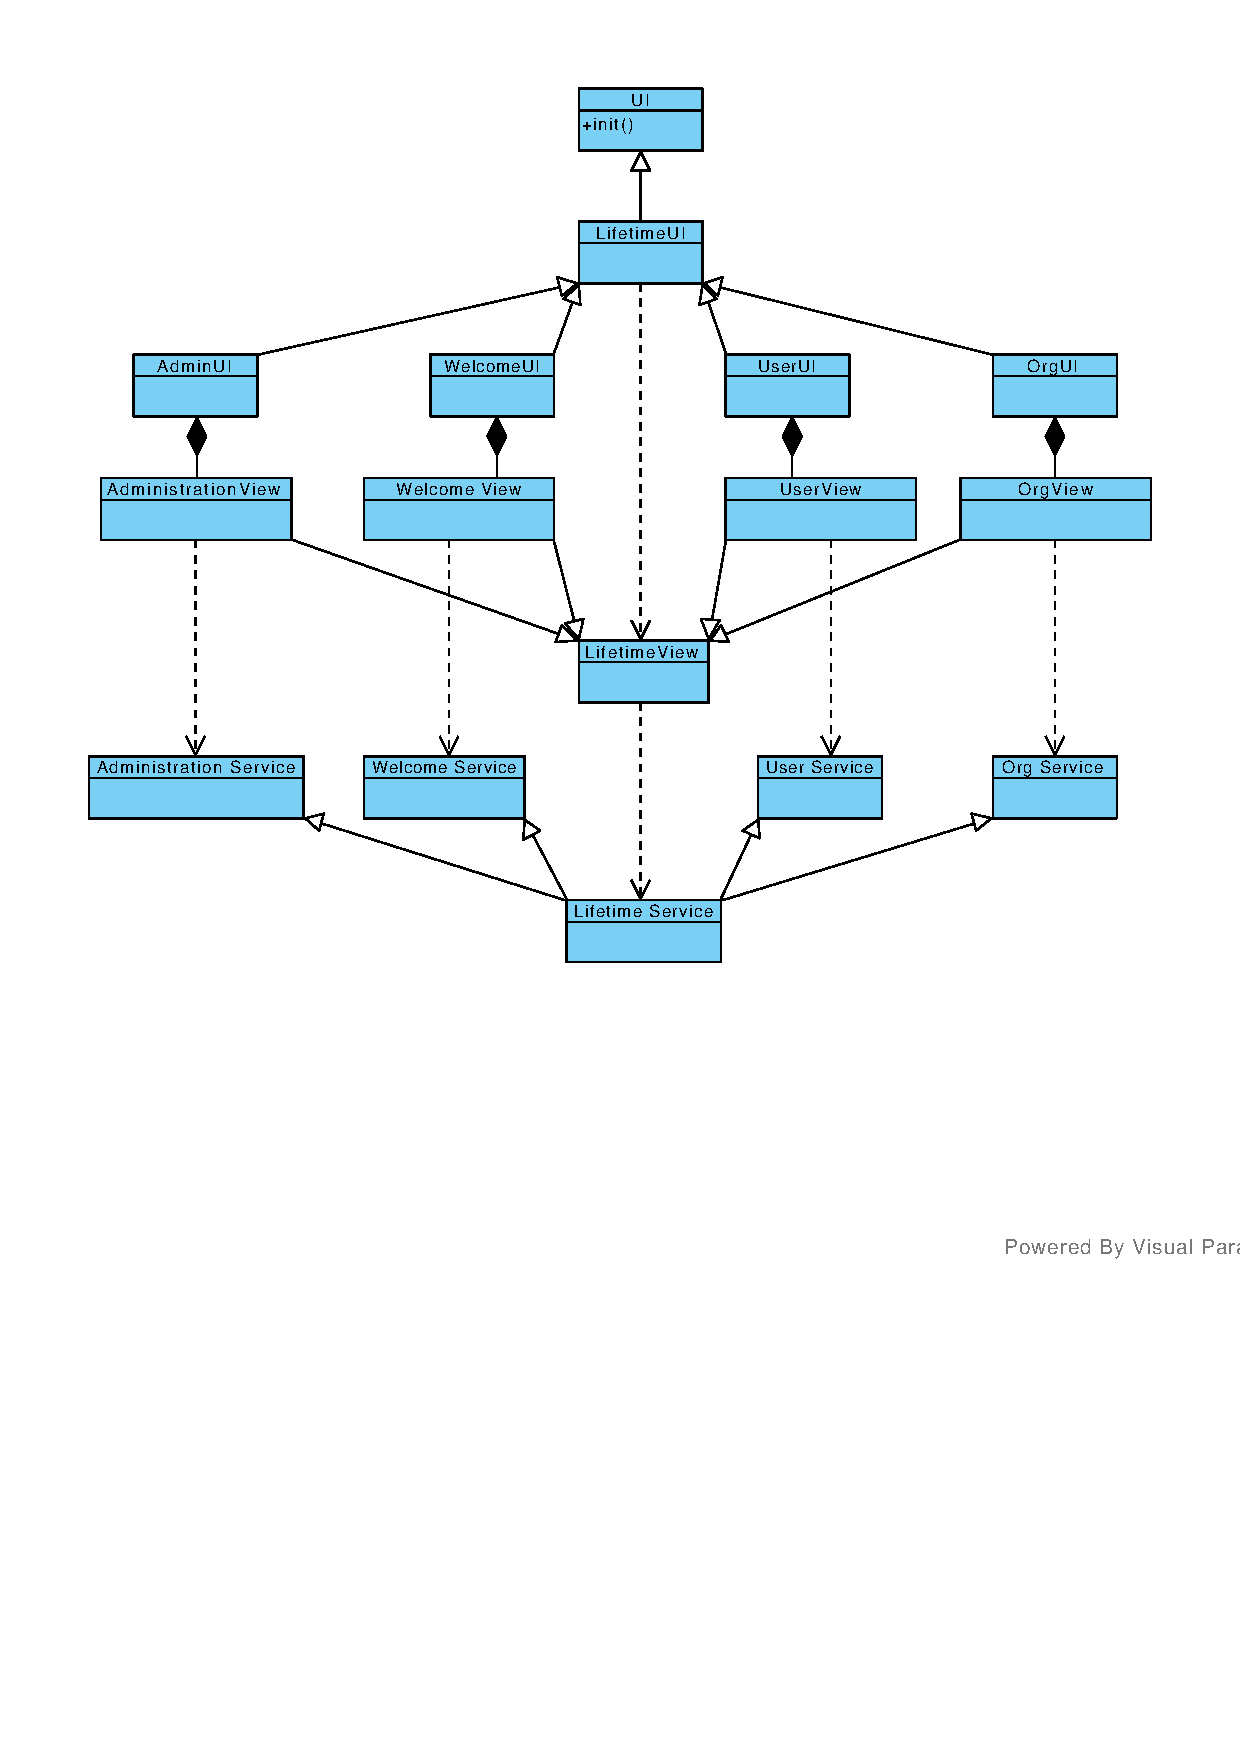
\includegraphics[scale=.75]{figures/uis}
  \caption{\vitae Application UIs}
  \label{fig:uis}
\end{figure}


\subsection{Functional}
\label{sec:requirements}

\subsection{Security}
\label{sec:security}

\paragraph{Roles}

\subparagraph{Application Server Roles}

\subparagraph{Programatic Roles}

\subparagraph{Role Mapping}

\subparagraph{Service Access}

\subparagraph{Secure UIs}

\subparagraph{Unsecure UIs}

\paragraph{Services}

\subparagraph{Guest Services}
\subparagraph{Private Member Services}
\subparagraph{Corporal Member Services}
\subparagraph{Administration Services}
\subparagraph{Developer Services}






\subsection{Others}
\label{sec:requirements}





%%% Local Variables:
%%% mode: latex
%%% TeX-master: "main"
%%% End:
